\documentclass[a4paper,12pt,twoside]{article}
\usepackage{graphicx}
\graphicspath{{./images/}}
\usepackage{wrapfig}
\usepackage{pdfpages,caption,geometry} %enables you to add pdf and a caption

\usepackage{geometry}
\geometry{
  a4paper,
  total={170mm,257mm},
  left=20mm,
  top=40mm,
  bottom=30mm,
}

\usepackage{color, colortbl}
\definecolor{Gray}{RGB}{220,220,220}

\usepackage[dvipsnames]{xcolor}
\definecolor{OMDTZblue}{RGB}{0, 166, 225}
\definecolor{OMDTZyellow}{RGB}{253, 214, 14}
\definecolor{OMDTZgreen}{RGB}{19, 186, 42}

\usepackage{sectsty}
\sectionfont{\color{OMDTZblue}} 
\subsectionfont{\color{OMDTZblue}}
\subsubsectionfont{\color{OMDTZblue}}

\usepackage{caption}
\usepackage[font={color=OMDTZgreen,small,bf},figurename=Fig.,labelfont={small,it}]{caption}
\usepackage{subcaption} 

\usepackage[utf8]{inputenc}
\usepackage[english]{babel}
\usepackage{multirow}
\usepackage{multicol} % Allows multiple columns to be used on the fly

\usepackage{fancyhdr}
\pagestyle{fancy}
\fancyhf{}
%\lhead{\color{black} \leftmark}
%\rhead{\color{black} \rightmark}
\fancyfoot[LE]{\color{black} \thepage \hspace{5mm} \scriptsize The Ethical GEO Initiative}
\fancyfoot[LO]{\color{black} \thepage \hspace{5mm} \scriptsize The Ethical GEO Initiative}

\newcommand*{\vcenteredhbox}[1]{\begingroup
\setbox0=\hbox{#1}\parbox{\wd0}{\box0}\endgroup} % For creating vertically centered rows of logos

\setcounter{tocdepth}{2} % Table of Contents includes only sections and subsections, not subsubsections.

\usepackage[framemethod=tikz]{mdframed}% adding a shadow to a text for emphasis
\usepackage{lipsum}

\usepackage{hyperref}
\hypersetup{
  colorlinks=true,
  linkcolor=OMDTZblue, % to match the OMDTZblue text
  filecolor=magenta,      
  urlcolor=cyan,
  pdftitle={The Ethical GEO Initiative},
  bookmarks=true,
  %pdfpagemode=FullScreen,
}
%\urlstyle{same}


\usepackage[english,ngerman]{babel}
\usepackage[T1]{fontenc}% font package

\usepackage[scale=1]{helvet} % or tgheros
\renewcommand{\familydefault}{\sfdefault}

\usepackage{bbding}% used for adding symbols e.g. checkmark


\begin{document}
\thispagestyle{empty}

\begin{center}
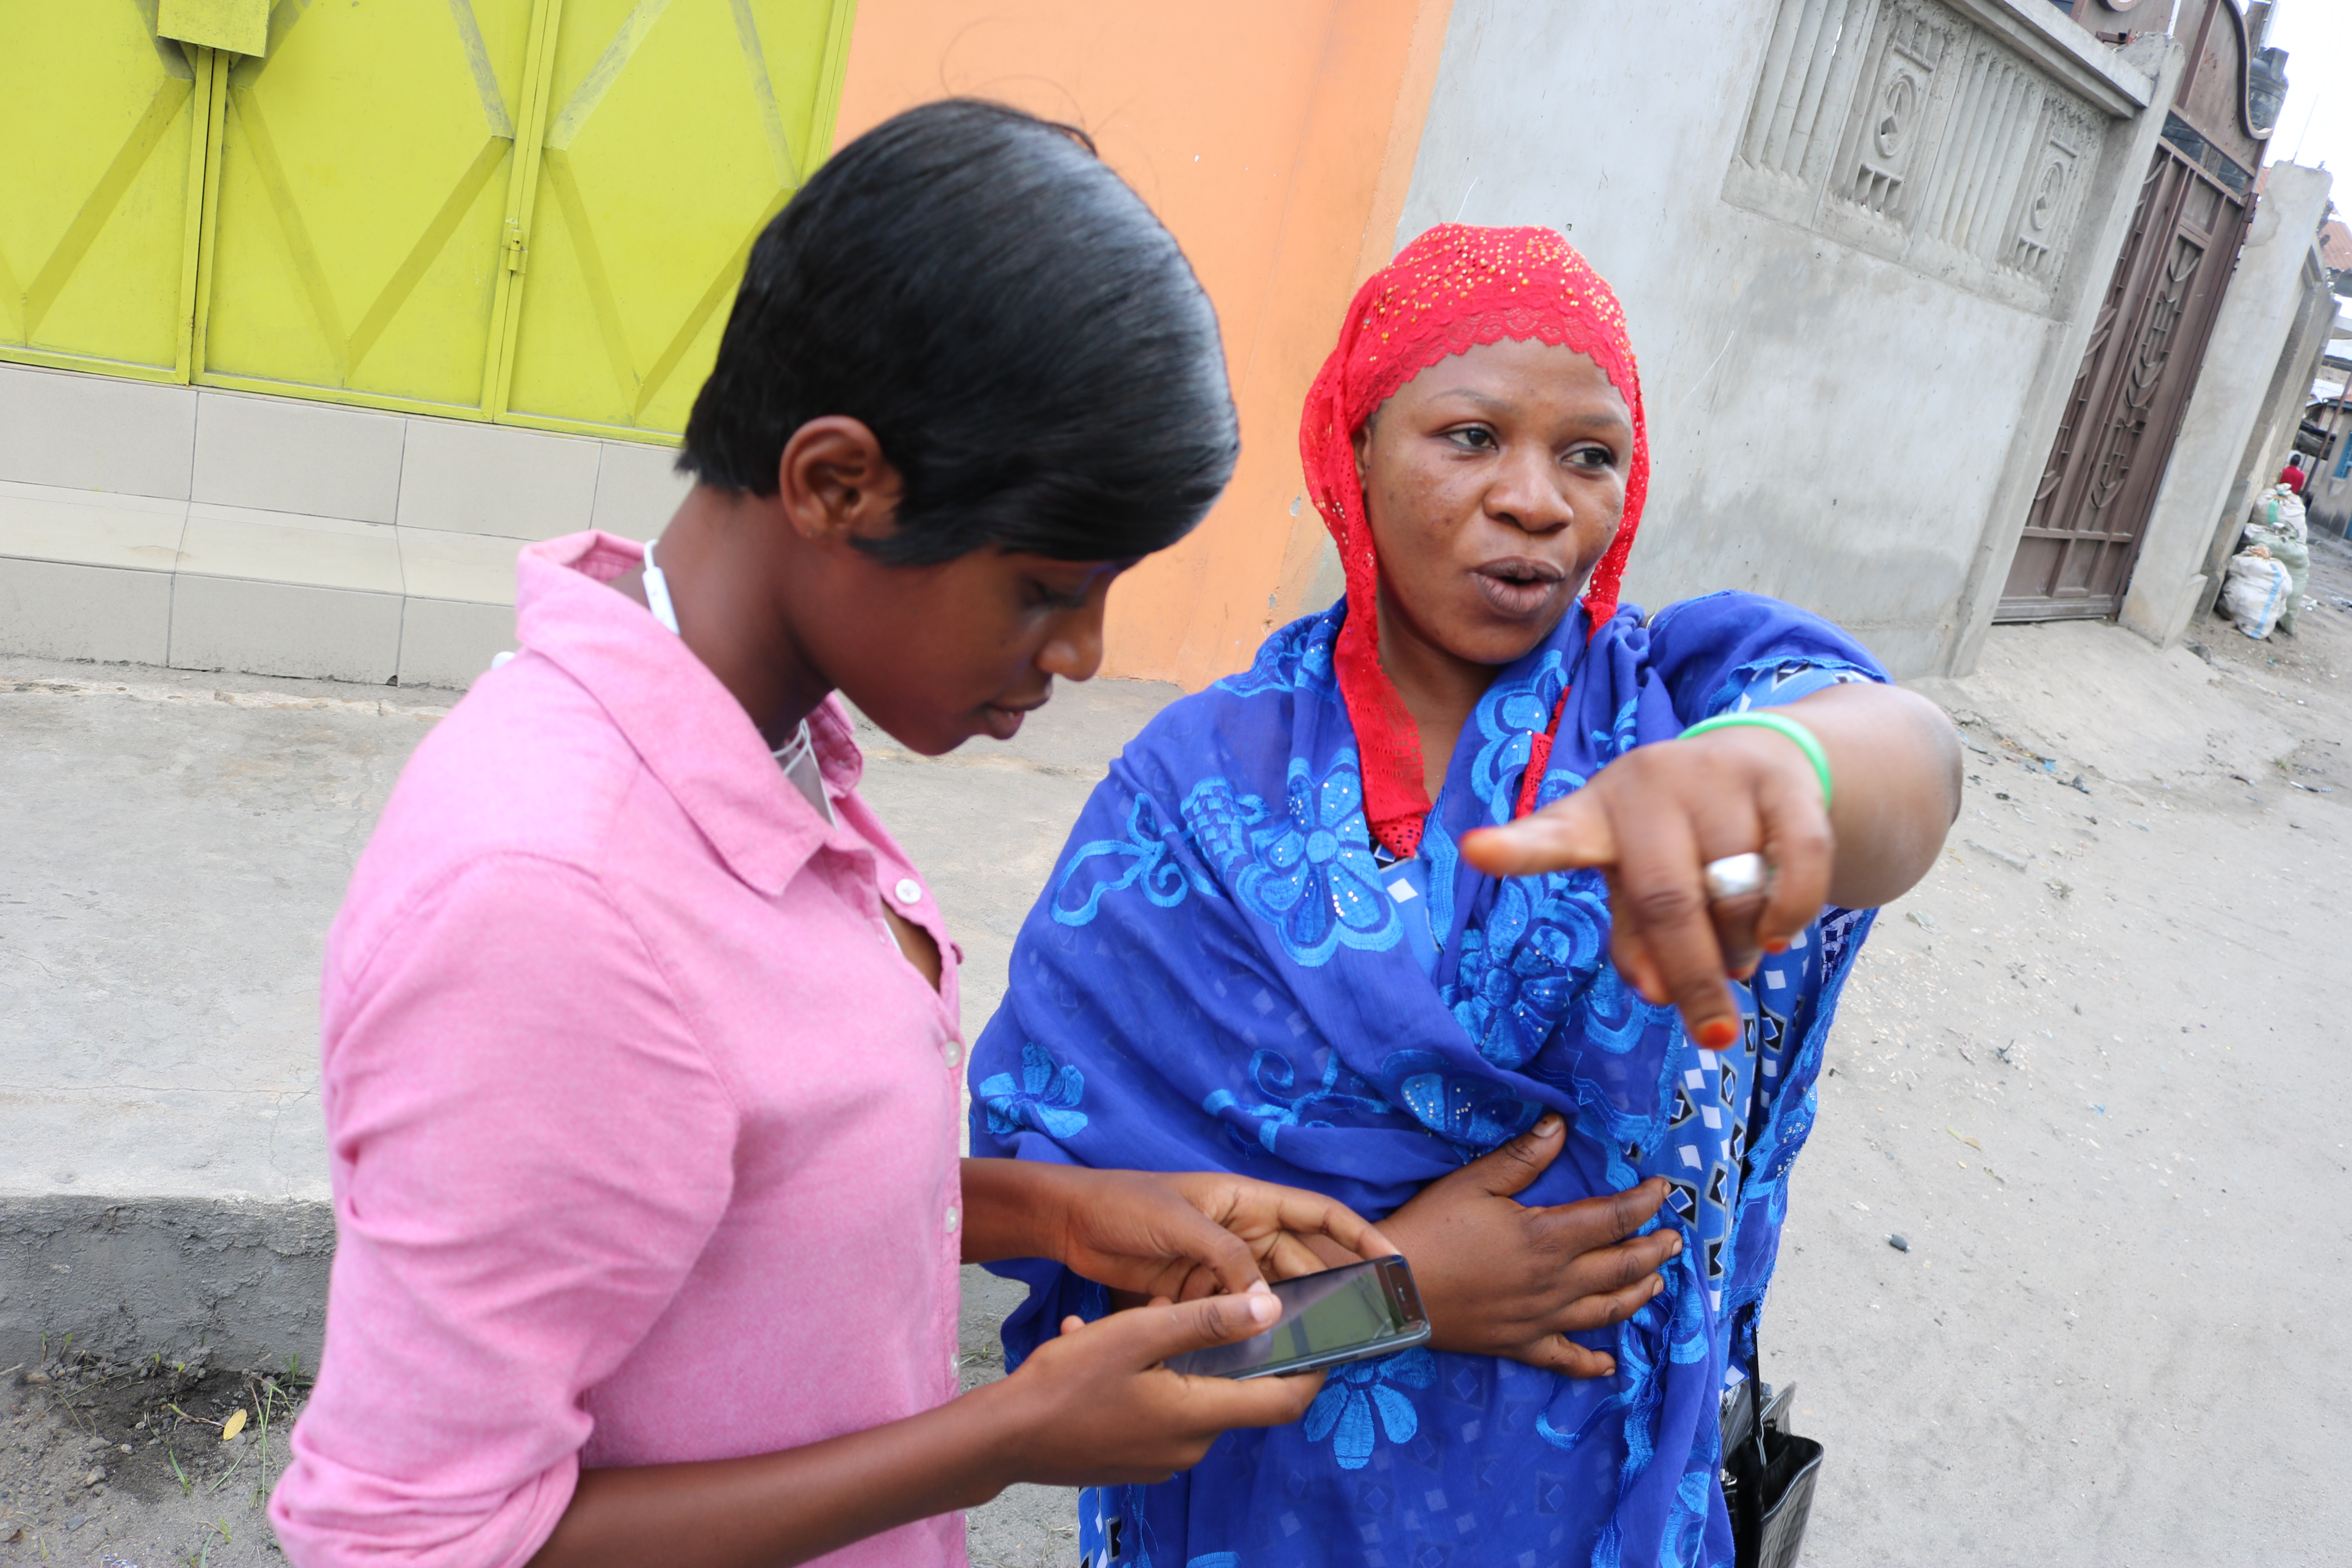
\includegraphics[width=\textwidth]{shina.jpg}
\end{center}

\begin{center}
\bigskip
  \Huge 
\color{OMDTZblue} \textbf {Land Rights for Informal Settlements in Dar es Salaam, Tanzania}

\\
\end{center}
\bigskip \bigskip \bigskip
\\
  \vbox{
  \centering
 
  By: {William Perry Evans}

  % \maketitle
}
\bigskip  \bigskip \bigskip
\begin{center}
  August 2019 
  
 \bigskip \bigskip \bigskip \bigskip \bigskip \bigskip
 
\footnotesize {Supported by: Deodatus Agricola, Benedcto Adamu, Immaculata Mwanja, Hawa Adinani, Godfrey Kassano}
  
\end{center}

\newpage
\fancyhead[L]{Land Rights for Informal Settlements in Dar es Salaam, Tanzania}
\section{Introduction}
On the Eastern coast of Tanzania lies Dar es Salaam, one of Africa’s fastest-growing urban centers. Experts project that it will achieve ‘megacity’ status in the next decade, with ten million residents or more. Of this population it is estimated that 70\% live in informal, unplanned settlements, subsisting on roughly a dollar per day. 
\bigskip

What this means is that these millions of residents do not have access to their land or property rights, depriving them of social stability. To put it bluntly, "A property without a land title is worthless,” says Tanzania’s Housing Minister, William Lukuvi. Obtaining a formal land title grants the owner access to credit, and provides essential protection to the urban poor. 
\bigskip

Herein lies the ethical challenge: How can Tanzanians living in informal settlements gain essential access to land tenure? This is just one piece of a much larger problem, as nearly a billion people worldwide live without legal title to their land. This is both a political as well as a technical challenge, where bureaucracy, as well as precise surveying, can be barriers. 
\bigskip

A key part of the solution is the use of new geospatial technology, in particular, dual-frequency receivers and open-source signal processing with mobile devices. This tech has only recently become affordable for the average citizen, and can help bridge the divide between the urban poor (who can’t afford surveys) and their land rights. Estimates show that this can drastically reduce the cost to families paying for their land titles, which become over a hundred times cheaper. 
\bigskip

What I propose for the EthicalGEO Initiative, is to use Real-Time Kinematics surveying with a newly released, low-cost, high-accuracy, dual-frequency sensor, to pave the way forward for land rights for the urban poor in Tanzania. Harnessing the power of this tech will be a local team of Tanzanian GIS experts, who will run a pilot project in Dar es Salaam. 


\section{Problem Statement}
At least 70\% of Dar es Salaam’s residents live in informal settlements with no access to their land rights. Rapid unplanned urbanization means the problem will only get worse in the years ahead. People are becoming increasingly vulnerable to health and environmental hazards such as dengue fever and annual flooding. 
\bigskip

The scale of the problem is huge, and in spite of efforts to address the problem, Tanzania is still listed as 146th most difficult country to register property, with 8 different procedures and a wait time of 67 days, according to a World Bank data collected in 2018. 
\bigskip

Besides these statistics, the reality is that most families cannot afford to pay the cost of mapping each plot, which the Minister of Lands reduced to 150,000 Tanzanian Shillings, or approximately \$65. This price is still far too high for the vast majority of informal residents. In addition, the professional surveyors who work in this field cannot afford to go through the process and create the survey for any less.
\bigskip

There have been different policies, strategies, and programs initiated by the Government of Tanzania to ensure all plots are surveyed and provided with title deeds through lowering the cost for plots survey, cost-sharing public housing programs, and slums upgrading among others - but still these strategies could not address the plot surveys needs which is huge in scale and is speeding up while informal settlements are expanding. 
\bigskip

In effect, this results in a Nash equilibrium whereby neither side can unilaterally succeed if the other remains unchanged. The transformative power of new geospatial technology can begin to solve the problem. I propose introducing it in a way that collaborates with existing surveyors, and works hand in hand with communities. 


\section{Main Goal and Objectives}
Main Goal: Make land rights accessible to the urban poor in Tanzania. 
\bigskip

Specific Objectives:
\bigskip

1. Conduct a pilot exercise in an informal subward of Dar es Salaam that provides cadastral surveys to one hundred community members
\medskip

2. Demonstrate the use of dual-frequency RTK and open source tools for reducing the cost of surveying
\medskip

3. Show the benefit of providing land rights to a single community, with a clear pathway to scale the project for the entire city
\medskip


\section{Cadastre Processes}

The history of cadastral surveys in Tanzania goes back to when it was under colonial rule - by Germany from 1890-1914, and then Britain from 1919-1961. Surveys served the colonial settlers by securing their land boundaries, whereas following independence the primary objective was to provide geometric descriptions for equitable access to land and the registration of land rights.
\bigskip

The basic unit of cadastral surveys is the land parcel - mapping of these land parcels provides a foundation to the cadastral survey system.  Chapter 324 of the Land Survey Act of Tanzania, Part I (2) states “cadastral survey means any survey the purpose of which is to obtain information for recording the position of the boundaries of lands in separate ownership or intended to be the subject of any disposition or partition, or re-establishing such boundaries on the ground or setting out new boundaries on the ground”.
\bigskip

In urban areas these are known as town plans. The three basic steps to conducting a cadastral survey in Tanzania are the request, execution, and submission - taken together these represent at least 8 different steps from the start to the end of the process. 
\bigskip

The importance of cadastral surveys cannot be understated - it is among the primary sources of land and resource property rights. They are meant to be, “simple, quick and affordable to speed up official access to secure land tenure by many citizens.” However, this goal is difficult to achieve when the cost of surveying is known to be high, and the amount of town plans needed is vast. 
\bigskip

All of the above has compounded the problem for the 70\% of people in Dar es Salaam that live in informal settlements. Some of the main challenges are lack of funding, the time required to create a town plan, and bureaucracy. Professional surveyors are using Real-Time Kinematics tools, which allow the user to obtain highly accurate (centimeter-level) positioning in real time. Still, the sensors they are using are significantly more expensive than the sensor being introduced for the first time in this project. 
\bigskip

The complexities inherent in the current cadastral surveying system in Tanzania make it such that poor people can rarely, if ever, obtain proper land rights. By using the latest tech with a local team I propose we change that.  

\section{Technology and Team}

A recent sensor has come to the market that allows its users to establish affordable, centimeter-precision location. The Swiss company U-blox has released a dual frequency GPS sensor, along with a dual frequency antenna, for under \$300. Tests done as recently as August 2019 show an accuracy of 2cm within Dar es Salaam. 
\bigskip

The RTK system (rover and base) works in combination with a simple Arduino and local Android phones. The output we have seen is astounding, and we believe it has may not only empower Tanzanians, but potentially a billion people worldwide who are living without land rights. 
\bigskip

To carry out this project I am partnering with OpenMap Development Tanzania (OMDTZ), a local non-governmental organization focused on mapping and open data. They are a team of roughly 15 Tanzanians, who have worked for years digitizing Dar es Salaam, and producing some of the best maps for resilience in the city. As a partner of Humanitarian OpenStreetMap Team (HOT), they have successfully carried out the Ramani Huria project funded by the World Bank since 2015. 


\section{Conclusion}

Across the world there are a billion people without legal titles to their land. We now have the tools to change that. There are doubtless to be significant barriers in the way, as new technology often disrupts old systems. We approach this with cultural and political sensitivity, as people well aware of the many ethical dimensions. 
\bigskip

The Ethical GEO Initiative is looking for the next big ideas using geospatial technology that spus conversation and keeps ethics at the forefront. In Tanzania, there are millions of people living without land rights, deprived of that basic social security that many in the West take for granted. 
\bigskip

With this project, I plan on using this fellowship to carry out a pilot in Dar es Salaam to benefit a local informal community. As a humanitarian practitioner, I am focused on underserved areas of the world, but in such a way that empowers local people. That is why I am submitting this proposal in partnership with a local organization, and plan on using the funds from the fellowship to work collaboratively with them to make it a reality.
\bigskip

As an American Geographical Society EthicalGEO Fellow, I would be honored to carry the conversation forward. 


\end{document}


%\begin{figure}
%\includegraphics[width=\columnwidth]{images/Asset&Threat.pdf}
%\caption{Image A}
%\end{figure} for adding .pdf files